\documentclass[11pt]{article}
\usepackage{calc}
\usepackage{color}
\usepackage{amsfonts}
\usepackage{latexsym}
\usepackage{placeins}
\usepackage{hyperref}
\usepackage[a4paper,top=5.5cm,bottom=4cm,left=2.5cm, right=2.5cm,foot=1cm]{geometry}
\pagenumbering{gobble}
\usepackage{setspace,relsize}               
\usepackage{moreverb}                        
\usepackage{url}
\hypersetup{colorlinks=true,citecolor=blue}
\usepackage{mathtools} 
\usepackage{amsthm}
\usepackage{amssymb}
\usepackage{indentfirst}
% \usepackage{todonotes}
\usepackage{subfigure}
\usepackage[numbers,square]{natbib}
\bibliographystyle{plain}
\usepackage[pdftex]{lscape}
\usepackage{authblk}
\usepackage{amsmath}
\usepackage[cp1250]{inputenc}
\usepackage[OT4]{fontenc}

\addtolength{\voffset}{-3.5cm} \addtolength{\textheight}{4cm}

\renewcommand{\refname}{\large{\textbf{ Bibliography}}}
\renewcommand\Authfont{\scshape\small}
\renewcommand\Affilfont{\itshape\small}
\newcommand{\keywords}[1]{\noindent{\large{\bf Keywords:}} #1\\}
\setlength{\affilsep}{1em}
\newcommand{\smalllineskip}{\baselineskip=15pt}
\newcommand{\emailaddress}[1]{{\sf#1}}
\newcommand{\speaker}[1]{\author{\underline{#1}}}
\newcommand{\speakeraffil}[1]{\affil{#1}}
\let\LaTeXtitle\title
\renewcommand{\title}[1]{\LaTeXtitle{\Large{\textbf{#1}}}}

% Title Page
\title{Some remarks on the uncertainty analysis of ${\cal R}_0$ in the SIR model}

\speaker{Luiz Max F. de Carvalho} % Write speaker name here

\author[1]{Daniel A. M. Villela}
\author[2]{Flavio Coelho}
\author[1]{Leonardo S. Bastos}

%%AFFILIATIONS
\speakeraffil{Program for Scientific Computing (PROCC), Oswaldo Cruz Foundation, Brazil,\,\emailaddress{lmax.procc@gmail.com}} % Write affiliation/s of the speaker here.

\affil[2]{School of Applied Mathematics, Getulio Vargas Foundation (FGV), Brazil,\,\emailaddress{fccoelho@fgv.br}} % Write affiliation/s of the first co-author here, if there is any. If not, remove the line.

\date{\vspace{-6ex}} % Do not modify this line


\DeclareMathOperator*{\argmin}{arg\,min}
\DeclareMathOperator*{\argmax}{arg\,max}
\newtheorem{theo}{Theorem}[]
\newtheorem{proposition}{Proposition}[]
\newtheorem{rmk}{Remark}[]
\setcounter{theo}{0} % assign desired value to theorem counter
\begin{document}
\maketitle

\begin{abstract}

Key-words: Basic reproductive number; uncertainty; logarithmic pooling; Gamma ratio distribution; . 
\end{abstract}

\section{Background}

${\cal R}_0$ is important, a key quantity in epidemic modelling.

Acknowledging uncertainty on parameter values is important.

logarithmic pooling is a nice and robust way of combining multiple sources of info.
\cite{poole2000} discuss the issue of propagating uncertainty through a deterministic model.


This begs the question, however, of in which order the pooling and propagation (inducing) operations should be performed.


\subsection{SIR model}

\begin{eqnarray*}
\frac{dS}{dt}&=& - \beta SI\\
\frac{dI}{dt}&=&  \beta SI - \gamma I\\
\frac{dR}{dt}&=& \gamma I 
\end{eqnarray*} 
where  $S(t) + I(t) + R(t) = N \quad \forall t$, $\beta$ is the transmission (infection) rate and $\gamma$ is the recovery rate.

\begin{equation}
\label{eq:r0def}
{\cal R}_0 = \frac{\beta N}{\gamma}. 
\end{equation}

\subsection{Uncertainty analysis}

$p(\beta, \gamma)$

$M(\cdot)$

$M(p(\beta, \gamma)) = p({\cal R}_0)$

For simplicity we will assume that $p(\beta, \gamma) = p(\beta)p(\gamma)$.

uncertainty about parameters can be represented by Gamma distributions.
\begin{eqnarray*}
f_{\beta}(b) &=& \frac{1}{\Gamma(k_1)\theta_1^{k_1}} b^{k_1} exp (- \frac{b}{\theta_1} ) \\
f_{\gamma}(g) &=& \frac{1}{\Gamma(k_2)\theta_2^{k_2}} g^{k_2} exp (- \frac{g}{\theta_2})
\end{eqnarray*}

\subsection{Logarithmic pooling} 

Logarithmic pooling is a popular method for combining opinions on an agreed quantity, specially when these opinions can be framed as probability distributions.
Let $\mathbf{F(\theta)} := \{f_1(\theta), f_2(\theta), \ldots, f_K(\theta)\}$ be a set of distributions representing the opinions of $K$ experts and let $\mathbf{w} :=\{w_1, w_2, \ldots, w_K \}$ be the vector of weights, such that $w_i > 0\: \forall i$ and $\sum_{i=0}^K w_i = 1$.
The \textbf{logarithmic pooling operator} $\mathcal{LP}(\mathbf{F(\theta)}, \mathbf{w})$ is defined as
\begin{equation}
\label{eq:logpool}
 \mathcal{LP}(\mathbf{F(\theta)}, \mathbf{w}) :=  \pi(\theta | \mathbf{w}) = t(\mathbf{w}) \prod_{i=0}^K f_i(\theta)^{w_i},
\end{equation}
where $t(\mathbf{w}) = \int_{\boldsymbol\Theta}\prod_{i=0}^K f_i(\theta)^{w_i}d\theta$.
This pooling method enjoys several desirable properties and yields tractable distributions for a large class of distribution families~\citep{genest1984, carvalho2016}.

\subsubsection{Induce-then-pool or pool-then-induce?}

Let $\theta \in \Theta \subseteq \mathbb{R}^p$ and $y \in \mathcal{Y} \subseteq \mathbb{R}^p$. 
Define the model (transformation) as $M \,:\, \Theta \to \mathcal{Y}$. 
This paper concerns the setting where a set $\mathbf{F(\theta)}$ of distributions on $\theta$ is available but one is interested in obtaining a pooled distribution on $y$.
There are two ways of obtaining a pooled distribution $\pi(y)$: (a) combine the distributions in $\mathbf{F(\theta)}$ and then apply $M(\cdot)$ to the resulting distribution to get the \underline{induced} distribution on $y$ (``pool-then-induce'') or; (b) apply  $M(\cdot)$ to each component of $\mathbf{F(\theta)}$ and combine the resulting induced distributions using the logarithmic pooling operator (``induce-then-pool''). 
First we note that under some conditions on the transformation $M(\cdot)$, the order in which one performs the pooling and transforming operations does not matter.
%% "Stolen" from http://math.stackexchange.com/questions/732960/inverse-of-a-multivariable-function
Consider $M(\theta) = y$ and suppose $M(\cdot)$ is invertible, i.e., there exists $M^{-1}: \: \mathcal{Y} \to \Theta$ such that,
\[A_0:\quad M(M^{-1}(v)) = v,\: v \in \mathcal{Y}\: \text{and}\: M^{-1}(M(t)) = t, \: t \in \Theta \]
and $J := det \left[ \frac{\partial M^{-1}}{\partial y_1}, \frac{\partial M^{-1}}{\partial y_2}, \ldots, \frac{\partial M^{-1}}{\partial y_p}\right]$.
With some abuse of notation, define
\begin{equation}
 \label{eq:transfF}
 \mathbf{F^{-1}(y)} := \{f_1(M^{-1}(y))|J|, \, f_2(M^{-1}(y))|J|, \ldots, \, f_K(M^{-1}(y))|J|\}
\end{equation}
where $|a|$ denotes the absolute value of $a$.
\begin{rmk}
\label{rmk:invariance}
Define $\pi_{\theta}(\theta | \mathbf{w}) =  \mathcal{LP}(\mathbf{F(\theta)}, \mathbf{w})$ and $\pi_{y}(y |\mathbf{w}) = \pi_{\theta}(M^{-1}(y))|J|$.
Similarly, define $\pi^{\prime}_{y}(y|\mathbf{w}) = \mathcal{LP}(\mathbf{F^{-1}(y)}, \mathbf{w})$.
If $A_0$ is satisfied, then $\pi_{y}(y |\mathbf{w}) = \pi^{\prime}_{y}(y|\mathbf{w})$, i.e., the order in which one combines and transforms the distributions does not matter.
\end{rmk}
\begin{proof}
To see that Remark~\ref{rmk:invariance} holds we only need a straightforward calculation from the definition of the logarithmic pooling operator in~(\ref{eq:logpool}):
\[\pi_{y}(y |\mathbf{w}) \propto \prod_{i=0}^K f_i(M^{-1}(y))^{w_i}|J| \]
whereas
\begin{align*}
 \pi^{\prime}_{y}(y|\mathbf{w}) &\propto  \prod_{i=0}^K \left[ f_i(M^{-1}(y))|J| \right] ^{w_i} = \prod_{i=0}^K f_i(M^{-1}(y))^{w_i} \prod_{i=0}^K|J|^{w_i}\\
 &\propto  \prod_{i=0}^K f_i(M^{-1}(y))^{w_i}|J|, %TODO: maybe = instead of \propto ?
\end{align*}
as claimed.
%% LM: if this embarassingly simple ``proof'' does not convince you, take a look at https://github.com/maxbiostat/R0_uncertainty/blob/master/code/invertible_model_equivalence.r
This is very similar in nature to the ``external Bayesianity'' property of the logarithmic pooling operator, by which one can either pool the prior distributions and then combine the resulting distribution with the likelihood or combine each prior with the likelihood separately and then pool the resulting posteriors to obtain the same posterior distribution.
%% TODO: if we can show that combining the prior with the likelihood is an invertible transform, then this result is a generalisation of EB. But we first need to see the degree of generality EB was actually proven in the original paper.
\end{proof}


\subsection{The Gamma ratio distribution}

To derive the distribution, we begin by noting that for $N > 1$, the distribution of $\beta^{\ast} = \beta N$ is a Gamma distribution with parameters $k_1$ and $N\theta_1$.
Under the assumption of independence $p(\beta^{\ast}, \gamma) = p(\beta^{\ast})p(\gamma)$, thus
\begin{eqnarray}
% {\cal R}_0 &=& \frac{\beta^{\ast}}{\gamma}\\
{\cal R}_0 &=& \beta^{\ast}/\gamma\\
f_{{\cal R}_0}(r) &=& A \int_{0}^{\infty} \gamma(\gamma r)^{k_1 -1} e^{-\frac{\gamma r}{N\theta_1}} \gamma^{k_2 -1} e^{-\frac{\gamma}{\theta_2}} d\gamma \\
A &=& \frac{1}{\Gamma(k_1)(N\theta_1)^{k_1}\Gamma(k_2)\theta_2^{k_2}}
\end{eqnarray}
Rearranging, yields
\begin{eqnarray}
\label{eq:toint}
f_{{\cal R}_0}(r) &=& A \int_{0}^{\infty} r^{k_1 -1} \gamma^{k_1 + k_2 -1} e^{-B\gamma} d\gamma \\
        B  &=& \frac{\theta_2 r + N\theta_1}{N\theta_1\theta_2}
\end{eqnarray}

\begin{eqnarray}
\label{eq:density}
f_{{\cal R}_0}(r) &=& \phi\times\space r^{k_1-1} (\theta_2 r + N\theta_1)^{-(k_1 + k_2)} \\
% f_{{\cal R}_0}(r) &=& \phi\frac{r^{k_1-1}}{(\theta_2 r + N\theta_1)^{(k_1 + k_2)}}\\
\label{eq:normconst}
\phi &=&  \frac{(N\theta_1\theta_2)^{k1+k2}}{\mathcal{B}(k_1, k_2)(N\theta_1)^{k_1}\theta_2^{k_2} }
\end{eqnarray}
where $\mathcal{B}(a, b) = \Gamma(a + b)/\Gamma(a)\Gamma(b)$ is the Beta function  and $\phi$ is the normalisation constant.
The probability distribution in~(\ref{eq:density}) will be called Gamma ratio distribution henceforth.
The expectation of the Gamma ratio distribution is then
\begin{align}
\label{eq:expR0}
E({\cal R}_0) &= \int_{0}^{\infty}rf_{R0}(r)dr \\
       &= \frac{N\theta_1}{\theta_2}\frac{k_1}{(k_2-1)}
\end{align}
and its variance can be computed as
\begin{eqnarray}
\label{eq:var1}
Var({\cal R}_0) &=& E({\cal R}_0^2) - E({\cal R}_0)^2  \\
\label{eq:var2}
 &=& \left(\frac{N\theta_1}{\theta_2}\right)^2\frac{(k_1+k_2-1)k_1}{(k_2-2)(k_2-1)^2}
\end{eqnarray}
which only exists for $k_2 > 2$.

The mode is 
\begin{equation}
\label{eq:mode}
\frac{N\theta_1}{\theta_2}\frac{k_1 - 1}{(k_2 + 1)}
\end{equation}
For a slightly different derivation, based on generalised Gamma distributions, see~\cite{Coelho2007}.

Now suppose we have two sets of prior probability distributions -- elicited by the same $K$ experts -- on $\beta$ and $\gamma$, $\mathbf{F}(\beta)$ and $\mathbf{G}(\gamma)$, respectively.
We will consider that all distributions for $\beta$ and $\gamma$ are Gamma distributions, parametrised as above.
Thus, for instance, the parameter $\theta_{2i}$ is the the scale parameter of the prior for the recovery rate ($\gamma$) given by the $i-$th expert.
Analogous to the above, assume the experts have a vector $\mathbf{w}$ of weights associated with them.
Suppose further that the components of these sets are independent, i.e., $p_i(\beta, \gamma) = f_i(\beta)g_i(\gamma)\: \forall i$.
One can either:
\begin{itemize}
 \item[(a)] construct $\pi(\beta | \mathbf{w}) = \mathcal{LP}(\mathbf{F}(\beta), \mathbf{w})$ and $\pi(\gamma | \mathbf{w}) = \mathcal{LP}(\mathbf{G}(\gamma), \mathbf{w})$ and then apply the transform in~(\ref{eq:r0def}) to obtain $\pi({\cal R}_0| \mathbf{w})$ or;
 \item[(b)] apply the transform to each component $i$ of $\mathbf{F}(\beta)$ and $\mathbf{G}(\gamma)$ to build
 \[\mathbf{R}({\cal R}_0):= \{r_i({\cal R}_0), r_2({\cal R}_0), \ldots, r_K({\cal R}_0)\} \]
 and obtain $\pi^{\prime}({\cal R}_0|  \mathbf{w}) = \mathcal{LP}(\mathbf{R}({\cal R}_0),  \mathbf{w})$.
\end{itemize}
Notice that the transform in~(\ref{eq:r0def}) is not invertible, and thus does not enjoy the property discussed in Remark~\ref{rmk:invariance}.
This means that in general, pooling-then-inducing (a) will yield a different distribution than inducing-then-pooling (b).
In fact, procedure (a) will lead to
\begin{equation}
 \pi_{{\cal R}_0}(r| \mathbf{w}) \propto   r^{k_{1}^{\ast}-1} (\theta_{2}^{\ast} r + N\theta_{1}^{\ast})^{-(k_{1}^{\ast} + k_{2}^{\ast})}
\end{equation}
where $k_{1}^{\ast} = \sum_{i=0}^K w_ik_{1i}$,  $k_{2}^{\ast} = \sum_{i=0}^K w_ik_{2i}$,  $\theta_{1}^{\ast} = \sum_{i=0}^K w_i\theta_{1i}$ and  $\theta_{2}^{\ast} = \sum_{i=0}^K w_i\theta_{2i}$.
The distribution resulting from procedure (b) will be 
\begin{align}
  \pi^{\prime}_{{\cal R}_0}(r| \mathbf{w}) &\propto   \prod_{i=0}^K \left[ r^{k_{1i}-1} (\theta_{2i} r + N\theta_{1i})^{-(k_{1i} + k_{2i})} \right]^{w_i} \\
   &\propto r^{k_{1}^{\ast}-1}  \prod_{i=0}^K (\theta_{2i} r + N\theta_{1i})^{-w_{i}(k_{1i} + k_{2i})}
\end{align}
where $k_{1}^{\ast}$ is defined as before.
An example plot of the resulting densities is shown in Figure~\ref{fig:transformAndKL}A.
We note that $\pi^{\prime}({\cal R}_0|  \mathbf{w})$ has thicker tails and therefore allows for more extreme values with higher probability.
This makes sense intuitively, because this distribution propagates uncertainty resulting from the model onto the final quantity.
% TODO: can we prove that [ItP has thicker tails] in general?
\begin{figure}
% \hfill
\begin{center}
\subfigure[][]{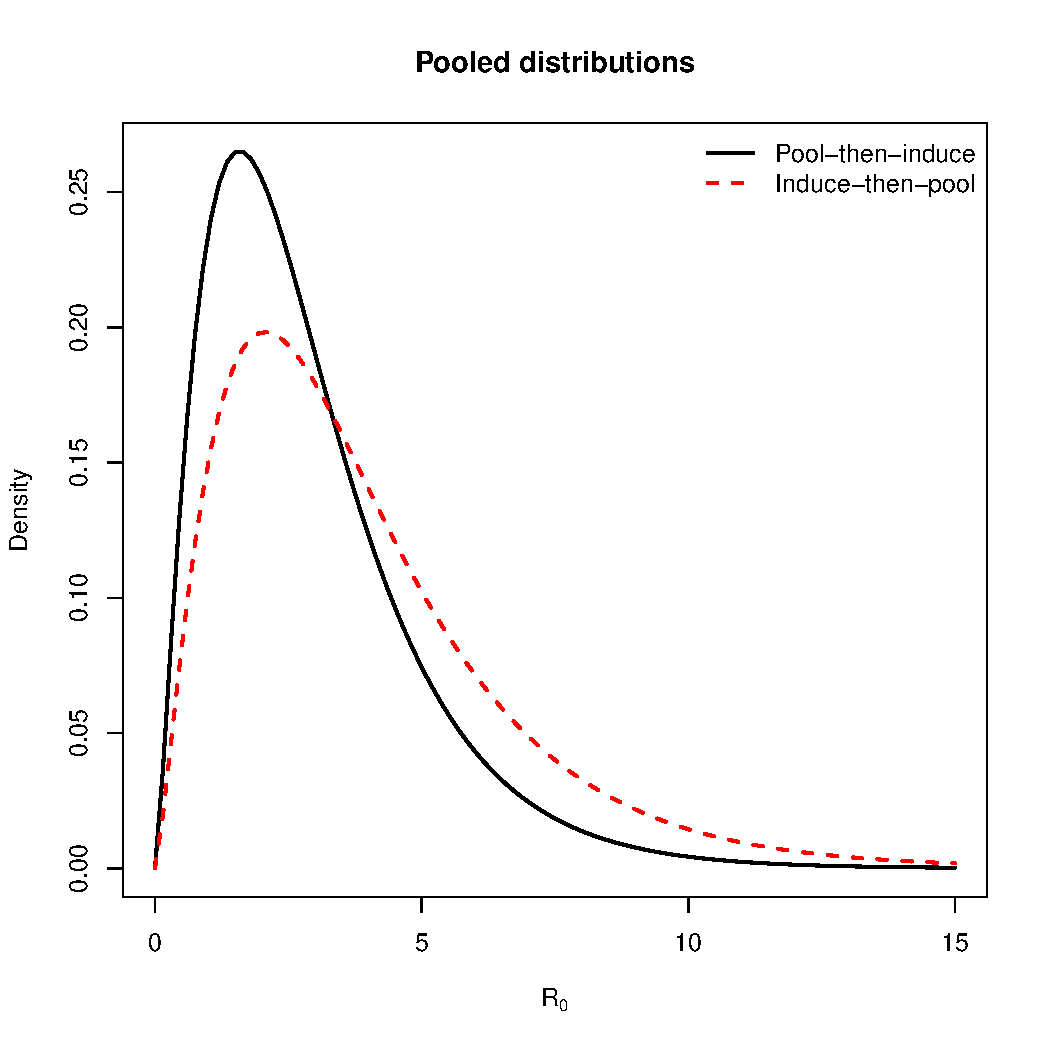
\includegraphics[scale=0.6]{figures/ItP_vs_PtI_equalWeights.pdf}} 
\end{center}
% \hfill
\begin{center}
\subfigure[][]{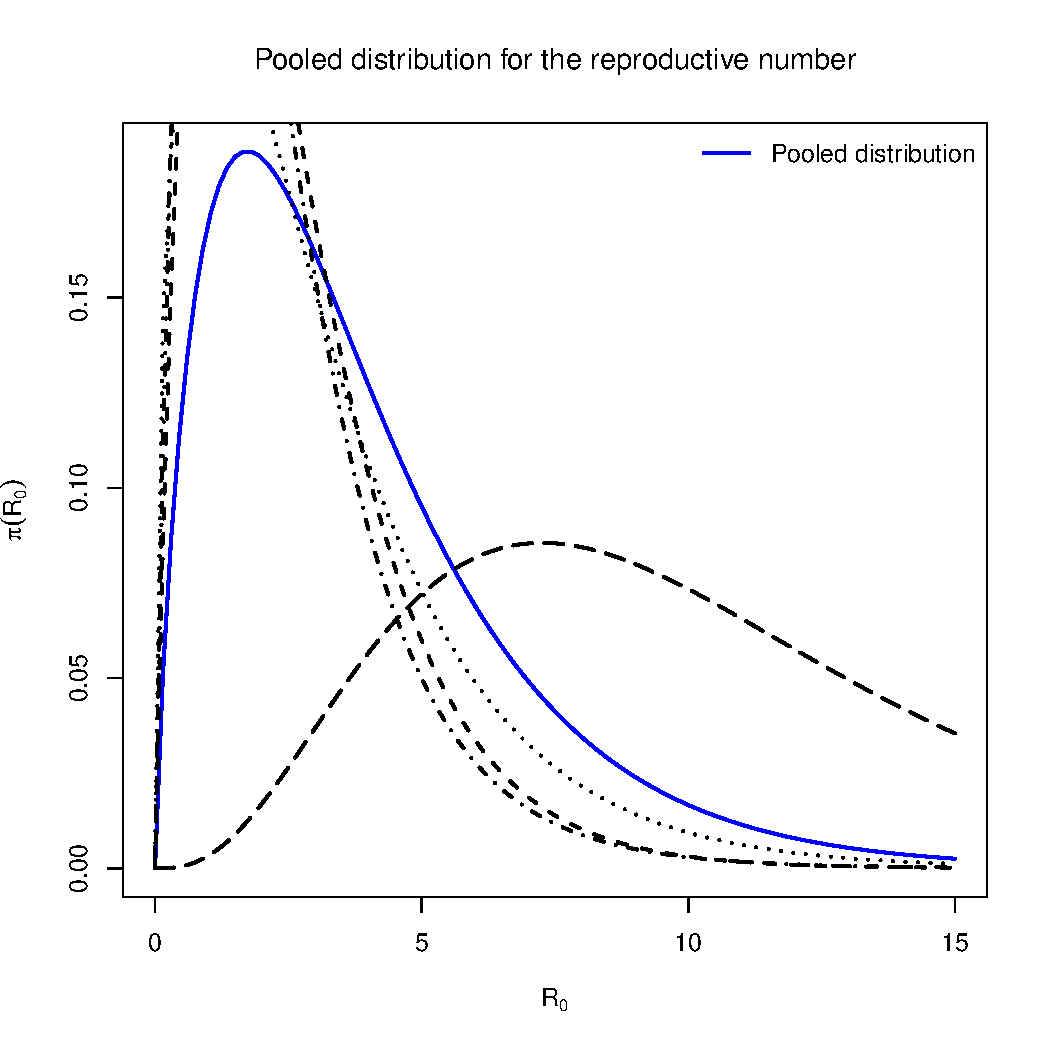
\includegraphics[scale=0.6]{figures/minKL_R0.pdf}} 
\end{center}
\caption{
\textbf{Distributions for ${\cal R}_0$}.
In panel A we present the `induce-then-pool'' and ``pool-then-induce'' distributions using equal weights ($\alpha_i = 1/K \:, \forall i$).
Panel B shows the pooled distribution for ${\cal R}_0$ that minimises KL divergence with the ``induce-then-pool'' distribution, i.e., that minimises discrepancy in transformed space.
}
\label{fig:transformAndKL}
\end{figure}

%% TODO: Compare the two (tails, concavity, etc) aka babble some moreverb
\section{Minimising Kullback-Leibler divergence in transformed space}


\section{Application: ${\cal R}_0$ for Ebola in West Africa}
[SCAN THE LITERATURE FOR BAYESIAN ESTIMATES]
\section*{Acknowledgements}
\bibliography{R0}
% \begin{figure}[!ht]
% \centering
% \includegraphics[width=\textwidth, height = 15cm]{figures/}
% \caption{\textbf{}.
% }
% \label{fig:}
% \end{figure}
%%
% \begin{figure}
% \hfill
% \subfigure[Title A]{\includegraphics[width=5cm]{img1}}
% \hfill
% \subfigure[Title B]{\includegraphics[width=5cm]{img2}}
% \hfill
% \caption{\textbf{}.
% }
% \label{fig:}
% \end{figure}
\end{document}          
